%hello world
\let\negmedspace\undefined
\let\negthickspace\undefined
\documentclass[journal,12pt,onecolumn]{IEEEtran}
\usepackage{cite}
\usepackage{amsmath,amssymb,amsfonts,amsthm}
\usepackage{algorithmic}
\usepackage{graphicx}
\usepackage{textcomp}
\usepackage{xcolor}
\usepackage{txfonts}
\usepackage{listings}
\usepackage{enumitem}
\usepackage{mathtools}
\usepackage{gensymb}
\usepackage{comment}
\usepackage[breaklinks=true]{hyperref}
\usepackage{tkz-euclide} 
\usepackage{listings}
\usepackage{gvv}                                        
%\def\inputGnumericTable{}                                 
\usepackage[latin1]{inputenc}                                
\usepackage{color}                                            
\usepackage{array}                                            
\usepackage{longtable}                                       
\usepackage{calc}                                             
\usepackage{multirow}                                         
\usepackage{hhline}                                           
\usepackage{ifthen}                                           
\usepackage{lscape}
\usepackage{tabularx}
\usepackage{array}
\usepackage{float}
\usepackage{multicol}


\newtheorem{theorem}{Theorem}[section]
\newtheorem{problem}{Problem}
\newtheorem{proposition}{Proposition}[section]
\newtheorem{lemma}{Lemma}[section]
\newtheorem{corollary}[theorem]{Corollary}
\newtheorem{example}{Example}[section]
\newtheorem{definition}[problem]{Definition}
\newcommand{\BEQA}{\begin{eqnarray}}
\newcommand{\EEQA}{\end{eqnarray}}
\newcommand{\define}{\stackrel{\triangle}{=}}
\theoremstyle{remark}
\newtheorem{rem}{Remark}

% Marks the beginning of the document
\begin{document}
\bibliographystyle{IEEEtran}
\vspace{3cm}

\title{ASSIGNMENT 3}
\author{EE24BTECH11031 - Jashwanth}
\maketitle

\bigskip

\textbf{Question}: Draw a rough sketch of the curve $y = \sqrt{x-1}$ in the interval $\sbrak{1,5}$. Find the area under the curve and between the lines $x = 1$ and $x = 5$.\\
\solution
As the graph is always above $x$-axis, the area$\brak{A}$ is \\
\begin{figure}[h]
	\centering
	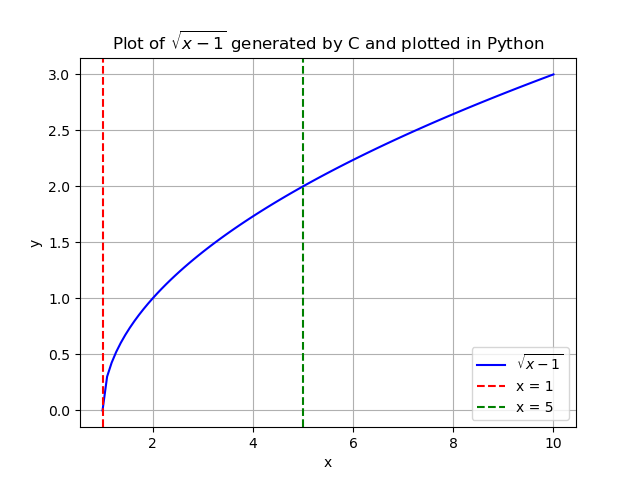
\includegraphics[scale=0.8]{figs/fig-1.png}
	\label{Fig}
\end{figure}
\begin{align}
	A &= \int_{1}^{5} \sqrt{x-1} dx\\
	A &= \sbrak{\frac{2}{3}{\brak{x-1}}^{\frac{3}{2}}}_{1}^{5}\\
	A &= \brak{\frac{2}{3}{\brak{5-1}}^{\frac{3}{2}}}-\brak{\frac{2}{3}{\brak{1-1}}^{\frac{3}{2}}}\\
	A &= \brak{\frac{2}{3}\times8}-\brak{\frac{2}{3}\times0}\\
	A &= \frac{16}{3}\\
\end{align}
Area under the graph is $\frac{16}{3}$.

\end{document}


